% fig_generalized: the generalized interdiction problem of BOBILib's set "generalized"
% (Fischetti, Monaci and Sinnl 2018), drawn schematically.
% Leader variables x (squares), follower variables y (circles).  For the first N pairs,
% x_j = 1 forces y_j = 0 (the follower's rows x_j + y_j <= 1).  The leader's rows
% G_x x + G_y y <= G_0 contain both x and y (coupling rows); the follower's own rows
% By <= b contain y only.  The objectives differ: the leader minimises c_x'x + c_y'y,
% the follower maximises d'y.  Shown: x_1 = 1 blocks y_1; x_4 = 1 is a leader decision
% that blocks nothing; the follower takes y_2 and y_5.  Schematic, no data.
% (In the files: rows inter<j> are x_j + y_j <= 1, rows leaderCons<i> are the leader's,
% rows followerCons<i> the follower's; each row also has a slack variable with a
% penalty of 100,000, which the figure leaves out.)
% Build: pdflatex fig_generalized.tex   (3.15 in x 1.75 in)
\documentclass[tikz,border=2pt]{standalone}
\pdfinfoomitdate=1 \pdftrailerid{} \pdfsuppressptexinfo=-1 % byte-identical rebuilds
\usepackage{mathptmx}
\usetikzlibrary{arrows.meta,calc}
\definecolor{leader}{HTML}{2A78D6}
\definecolor{follower}{HTML}{EB6834}
\definecolor{cert}{HTML}{1BAF7A}
\definecolor{ink}{HTML}{0B0B0B}
\definecolor{ink2}{HTML}{52514E}
\definecolor{muted}{HTML}{A9A8A2}
\definecolor{grid}{HTML}{E6E5E0}
\tikzset{
  every picture/.style={font=\fontsize{8}{9.6}\selectfont, color=ink, line cap=round, line join=round},
  small/.style={font=\fontsize{7}{8.4}\selectfont},
  lbox/.style={leader, line width=0.8pt, densely dashed, rounded corners=4pt},
  fbox/.style={follower, line width=0.8pt, rounded corners=4pt},
  link/.style={ink2, line width=0.7pt},
}
\begin{document}
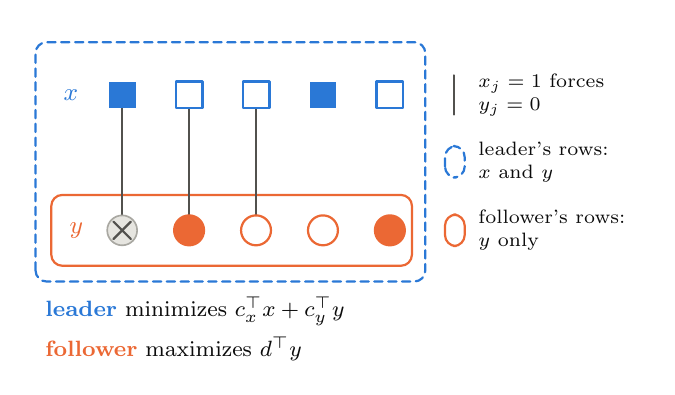
\begin{tikzpicture}
  % fixed page: 3.15 in x 1.75 in including the 2 pt border
  \useasboundingbox (0,0) rectangle (7.86,4.304);
  \def\yx{3.45}  % leader row
  \def\yy{1.73}  % follower row
  \def\s{0.17}   % half size of a square

  % rows of constraints
  \draw[lbox] (0.10,1.08) rectangle (5.05,4.12);
  \draw[fbox] (0.30,1.28) rectangle (4.88,2.18);

  % interdiction links for the first three pairs
  \foreach \i in {0,1,2} \draw[link] (1.20+0.85*\i,\yx-\s) -- (1.20+0.85*\i,\yy+0.20);

  % leader variables: x_1 and x_4 chosen (filled)
  \foreach \i/\f in {0/1,1/0,2/0,3/1,4/0} {
    \pgfmathsetmacro{\xx}{1.20+0.85*\i}
    \ifnum\f=1 \fill[leader] (\xx-\s,\yx-\s) rectangle ++(2*\s,2*\s);
    \else \draw[leader, line width=0.8pt, fill=white] (\xx-\s,\yx-\s) rectangle ++(2*\s,2*\s); \fi
  }
  % follower variables: y_1 blocked, y_2 and y_5 taken
  \draw[muted, line width=0.6pt, fill=grid] (1.20,\yy) circle (0.19);
  \draw[ink2, line width=0.8pt] (1.20-0.11,\yy-0.11) -- (1.20+0.11,\yy+0.11) (1.20-0.11,\yy+0.11) -- (1.20+0.11,\yy-0.11);
  \foreach \i/\f in {1/1,2/0,3/0,4/1} {
    \pgfmathsetmacro{\xx}{1.20+0.85*\i}
    \ifnum\f=1 \draw[follower, line width=0.8pt, fill=follower] (\xx,\yy) circle (0.19);
    \else \draw[follower, line width=0.8pt, fill=white] (\xx,\yy) circle (0.19); \fi
  }
  \node[text=leader, font=\fontsize{9}{10}\selectfont] at (0.55,\yx) {$x$};
  \node[text=follower, font=\fontsize{9}{10}\selectfont] at (0.62,\yy) {$y$};

  % objectives
  \node[anchor=west] at (0.10,0.70) {\textcolor{leader}{\bfseries leader} minimizes $c_x^\top x + c_y^\top y$};
  \node[anchor=west] at (0.10,0.22) {\textcolor{follower}{\bfseries follower} maximizes $d^\top y$};

  % key
  \begin{scope}[shift={(5.30,0)}, small]
    \draw[link] (0.12,3.70) -- (0.12,3.20);
    \node[anchor=west, align=left] at (0.30,3.45) {$x_j=1$ forces\\$y_j=0$};
    \draw[lbox] (0.0,2.40) rectangle (0.25,2.80);
    \node[anchor=west, align=left] at (0.30,2.60) {leader's rows:\\$x$ and $y$};
    \draw[fbox] (0.0,1.53) rectangle (0.25,1.93);
    \node[anchor=west, align=left] at (0.30,1.73) {follower's rows:\\$y$ only};
  \end{scope}
\end{tikzpicture}
\end{document}
